% THIS IS SIGPROC-SP.TEX - VERSION 3.1
% WORKS WITH V3.2SP OF ACM_PROC_ARTICLE-SP.CLS
% APRIL 2009
%
% It is an example file showing how to use the 'acm_proc_article-sp.cls' V3.2SP
% LaTeX2e document class file for Conference Proceedings submissions.
% ----------------------------------------------------------------------------------------------------------------
% This .tex file (and associated .cls V3.2SP) *DOES NOT* produce:
%       1) The Permission Statement
%       2) The Conference (location) Info information
%       3) The Copyright Line with ACM data
%       4) Page numbering
% ---------------------------------------------------------------------------------------------------------------
% It is an example which *does* use the .bib file (from which the .bbl file
% is produced).
% REMEMBER HOWEVER: After having produced the .bbl file,
% and prior to final submission,
% you need to 'insert'  your .bbl file into your source .tex file so as to provide
% ONE 'self-contained' source file.
%
% Questions regarding SIGS should be sent to
% Adrienne Griscti ---> griscti@acm.org
%
% Questions/suggestions regarding the guidelines, .tex and .cls files, etc. to
% Gerald Murray ---> murray@hq.acm.org
%
% For tracking purposes - this is V3.1SP - APRIL 2009

\documentclass{../dependencies/acm_proc_article-sp}

\usepackage{url}
\usepackage{color}
\usepackage{verbatim}
\usepackage{listings}
\usepackage{graphicx}
\lstset{
  language=C++,             % choose the language of the code
  basicstyle=\small,       % the size of the fonts that are used for the code
  numbers=left,                   % where to put the line-numbers
  numberstyle=\footnotesize,      % the size of the fonts that are used for the line-numbers
  stepnumber=0,                   % the step between two line-numbers. If it is 1 each line will be numbered
  numbersep=5pt,                  % how far the line-numbers are from the code
  backgroundcolor=\color{white},  % choose the background color. You must add \usepackage{color}
  showspaces=false,               % show spaces adding particular underscores
  showstringspaces=false,         % underline spaces within strings
  showtabs=false,                 % show tabs within strings adding particular underscores
  %frame=single,                   % adds a frame around the code
  tabsize=2,              % sets default tabsize to 2 spaces
  captionpos=t,                   % sets the caption-position to bottom
  breaklines=true,        % sets automatic line breaking
  breakatwhitespace=false,    % sets if automatic breaks should only happen at whitespace
  escapeinside={\%}{)}          % if you want to add a comment within your code
}


\begin{document}

\title{ Results Of Our Efforts To Improved MongoDB }
%
% You need the command \numberofauthors to handle the 'placement
% and alignment' of the authors beneath the title.
%
% For aesthetic reasons, we recommend 'three authors at a time'
% i.e. three 'name/affiliation blocks' be placed beneath the title.
%
% NOTE: You are NOT restricted in how many 'rows' of
% "name/affiliations" may appear. We just ask that you restrict
% the number of 'columns' to three.
%
% Because of the available 'opening page real-estate'
% we ask you to refrain from putting more than six authors
% (two rows with three columns) beneath the article title.
% More than six makes the first-page appear very cluttered indeed.
%
% Use the \alignauthor commands to handle the names
% and affiliations for an 'aesthetic maximum' of six authors.
% Add names, affiliations, addresses for
% the seventh etc. author(s) as the argument for the
% \additionalauthors command.
% These 'additional authors' will be output/set for you
% without further effort on your part as the last section in
% the body of your article BEFORE References or any Appendices.

\numberofauthors{3} %  in this sample file, there are a *total*
% of EIGHT authors. SIX appear on the 'first-page' (for formatting
% reasons) and the remaining two appear in the \additionalauthors section.
%
\author{
% You can go ahead and credit any number of authors here,
% e.g. one 'row of three' or two rows (consisting of one row of three
% and a second row of one, two or three).
%
% The command \alignauthor (no curly braces needed) should
% precede each author name, affiliation/snail-mail address and
% e-mail address. Additionally, tag each line of
% affiliation/address with \affaddr, and tag the
% e-mail address with \email.
%
% 1st. author
\alignauthor
Brian Gianforcaro \\
       \affaddr{RIT}\\
       \email{bjg1955@rit.edu}
% 2nd. author
\alignauthor
Joseph Schrama \\
       \affaddr{RIT}\\
       \email{jfs2776@rit.edu}
% 3rd. author
\alignauthor
Nicholas Williams \\
       \affaddr{RIT}\\
       \email{nxw6572@rit.edu}
}
\maketitle
\begin{abstract}
MongoDB is a state of the art document oriented database that
has emerged out of the NoSQL movement. MongoDB is scalable and
focuses on high performance. Although the database is packed with features,
some area's of it's implementation and interface leave's something to be
desired. We present multiple significant modifications to the MongoDB project
which enhance usability and overall functionality. Our enhancements range from
the area of geoSpatial search, to user authentication, and even expanding querying
syntax to support XPath like syntax.
We describe our success's as well as our failures in our journey to improve this
``Humongous'' database.
%the formatting guidelines for ACM SIG Proceedings.
%It complements the document \textit{Author's Guide to Preparing
%ACM SIG Proceedings Using \LaTeX$2_\epsilon$\ and Bib\TeX}. This
%source file has been written with the intention of being
%compiled under \LaTeX$2_\epsilon$\ and BibTeX.
%
%The developers have tried to include every imaginable sort
%of ``bells and whistles", such as a subtitle, footnotes on
%title, subtitle and authors, as well as in the text, and
%every optional component (e.g. Acknowledgments, Additional
%Authors, Appendices), not to mention examples of
%equations, theorems, tables and figures.
%
%To make best use of this sample document, run it through \LaTeX\
%and BibTeX, and compare this source code with the printed
%output produced by the dvi file.
\end{abstract}

%% A category with the (minimum) three required fields
\category{H.4}{Information Systems Applications}{Miscellaneous}
%%%A category including the fourth, optional field follows...
%
%\terms{Theory}

\keywords{ MongoDB, NoSQL, RIT, Database System Implementation, XPath, GeoSpatial Search, Building Index's in Parallel} % NOT required for Proceedings
%
%\footnotetext[1]{NoSQL databases, also known as structured storage are known for not requiring a fixed table schema and often avoid join operations. The thing that
% links them together is there use of alternate query languages from SQL.}

\section{Introduction}
Our group has chosen to work on MongoDB 
\footnote{MongoDB is an open source project which is produced by the 10gen corperation.
          Development is done in the open and the company sells suport and infrastructure for profit. }
          for our Database Systems
Implementation Project. MongoDB is a document oriented so-called NoSQL 
\footnote{ NoSQL is a relatively new term, which describes a family of databases that differ from the classical relational database managment system design and implementation. NoSQL databases are often schema-less and avoid join like operations for performance reasons }
database system. MongoDB databases have no schemata and strive to give the user
the fastest performance possible. Much of this is done through clustering/sharding
and a focus on concurrent algorithms. MongoDB has a variety of very unique
features which set it apart from other NoSQL or document oriented databases.
Instead of a traditional SQL syntax for interacting with the database, MongoDB uses
a new format known as BSON (Binary JavaScript Object Notation) which is very similar
to JSON ( JavaScript Object Notation ).
%\begin{lstlisting}
%
%{ "title":"Blog Post", "id":25, ... }
%\end{lstlisting}
The database kernel and the tools built for interacting with MongoDB are written in
C++. The kernel and tools heavily utilize object oriented design patterns.
However, the database embeds the Mozilla SpiderMonkey JavaScript engine.
Using this engine JavaScript can be written, stored and executed on the database server; these
operations are similar to stored procedures. MongoDB also has a specification for storing
large files under MongoDB, known as GridFS. GridFS is a standard for breaking up these larger
files and storing them efficiently, a user can then query ranges of the file. For example if the
database is storing a large MP3 file, the user can seek to the middle of it and the database can
efficiently seek to the relevant section.

MongoDB is rich with new and exciting features and is a completely open source project.
The database has an active developers mailing list as well as an excellent issue tracker,
wiki for documentation and IRC channel for help. With all of these resources and
the many features requested on the issue tracker, our group felt that MongoDB would be a great
project to work on this quarter. The database has also been gaining a lot of traction in the
database world. MongoDB will more than likely prove to be a very useful product
to have working knowledge of in the future.

\section{Results Of Our Improvements}
\subsection{Parallel Index Building}
In MongoDB, indexes are represented using B-Trees.
There exists a foreground index build operation and a "background" index build operation.
The former locks the entire database while the latter locks the shell from which the command was issued (but does not lock the entire database).
Due to these limitations, it seemed that multi-threading an index build operation would be beneficial.
When the foreground build operation is used, the B-Tree is bulk-loaded and built from the bottom up; the background build operation uses a slower technique\cite{1}.
The foreground operation begins by sorting the keys to make up the leaf level and then building the tree upwards from that level.
We predicted that we would be able to split the sorted keys between the threads and have each thread build a sub-tree.
We intended for the sub-trees to be combined together into the final tree once all of the threads had finished.
Because of this opportunity and the fact that the foreground operation seemed more useful than the background operation, we elected to only parallelize the foreground operation.
To merge the sub-trees back together, we attempted to adapt the algorithm used to build new levels in the B-Tree.
This approach allowed for the possibility of building more than one level on top of the sub-trees in order to form the final tree.
This was significantly complicated, especially considering the lack of commenting in the original code.
The latest attempt at this appears in a version of IndexChunkBuilder.mergeIndexSubTrees() which starts at line 1142 of db/pdfile.cpp.old.
We were unable to get this algorithm to merge the sub-trees.
We then attempted to perform the merge while only adding a single new level with a root node.
The code which was to perform this task appears in IndexChunkBuilder.mergeIndexSubTrees( This function starts at line 1148 of db/pdfile.cpp.
It would require an exceptionally large data set and an exceptional large number of threads of execution in order to take advantage of the earlier approach.
Whenever an index would be built, strange assertion statements would fail (e.g. assert(this) in an instance member).
Profiling indicated that this was happening before our attempt to merge the sub-trees together, while the sub-trees were being built on-disk.
We then discovered a message board posting which stated that MongoDB does not currently support parallel writes to a database\cite{2} (except in a certain distributed database setup)\cite{3}.
Given this, it would be virtually impossible to finish this extension.)

\subsection{Polygon Geospatial Seach}
Currenlty MongoDB has a fairly versatile 2D GeoSpatial search API.
The user has the ability to create a 2D BTree index on any numeric pair of points.

\begin{figure}[htb]
\centering
%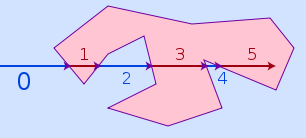
\epsfig{file=ray.eps}
\setlength\fboxsep{0.5pt}
\setlength\fboxrule{0.5pt}
\fbox{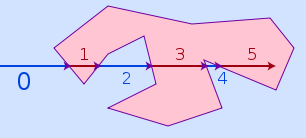
\includegraphics[scale=0.80]{ray.png}}
\caption{An example of a ray being cast across a polygon, computing the crossing number.}
\end{figure}
 

\begin{figure}[htb]
\centering
%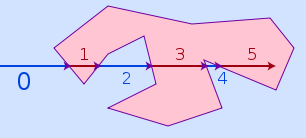
\epsfig{file=ray.eps}
\setlength\fboxsep{0.5pt}
\setlength\fboxrule{0.5pt}
\fbox{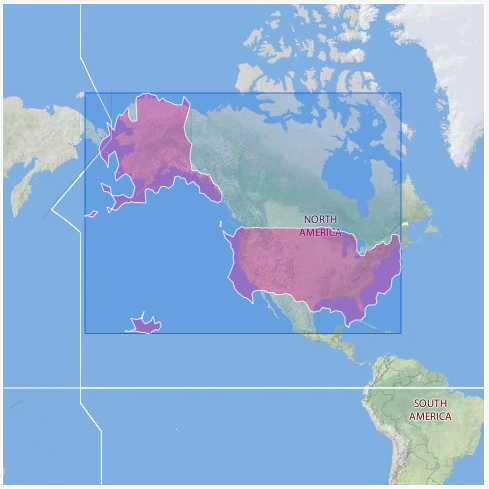
\includegraphics[trim = 25mm 50mm 25mm 25mm, clip, width=8cm]{map.jpg}}
\caption{An example of possible GeoSpatial search polygons for the different parts of the United States.}
\end{figure}
 
\subsection{Support for XPath-like Queries}
XPath is a very common query syntax for Document based structures. Since MongoDB uses a document-oriented data structure (BSON) for its database, it is only logical that MongoDB support XPath-like queries. The first step in adding support for XPath-like queries was adding the ability to use wildcards for sub-objects in the document hierarchy. This allows for the user to search a document for specific child objects-or nodes, as they are referred to in XPath-without specifying all its ancestors. For example, if you had a database containing the entries

\begin{lstlisting}

{ zoo : { location : { animal : {
    type : "zebra" , age : 0 } } } }
\end{lstlisting}

and

\begin{lstlisting}

{ zoo : { location : { animal : {
    type : "rhino" , age: 0 } } } }
\end{lstlisting}

in a collection named 'collection' and you wanted to find all animals in your database that are newborns (age equals 0), regardless of their location, you could find them with the wildcard query:

\begin{lstlisting}

db.collection.find({ "zoo.*.animals.age" : 0 })
\end{lstlisting}

This becomes increasingly beneficial as you develop larger and more complex data objects, since you can substitute any number of levels in the hierarchy with wildcards. The next step in adding support for XPath-like queries was allowing the user to pass said queries into the shell, as it currently only communicates with the server using BSON objects. To simplify things, we chose to convert the XPath query into the equivalent BSON object on the client side and simply pass that along to the server, allowing MongoDB to use its built-in mechanisms for querying the database. Given the time constraint for the project, we were not able to include an XPath-equivalent for the multitude of XPath and Mongo shell commands. We were, however, able to incorporate the following for our Phase 3 release:

\begin{itemize}
  \item	The use of XPath slash notation (represents object hierarchy in terms of absolute paths)
  \item	A number of comparators (>, >=, =, <, <=, !=)
  \item	The 'or' and 'and' operators (expressed as ' or ', ' and ', |, \&\&)
  \item	Returning indexed results-eliminating the need for Mongo's skip and limit functions in most cases
\end{itemize}

The greatest difficulties we faced with this part of the project was adding support for wildcard queries and finding the appropriate entry point for inserting our code to allow for, and convert from, XPath queries in the shell. Once we overcame these challenges, it was a simple matter of parsing the user's input.

The following are examples of typical MongoDB queries followed by their XPath equivalent.\footnote{Uses sample database set up using the build-database file specified in the P3 README}

Return the fourth animal in the zoo:
\begin{lstlisting}

db.test.find({ "zoo.animal" : { $exists : true } }).skip(3).limit(1)

db.test.find("/zoo/animal[4]");
\end{lstlisting}

Return all animals in the zoo of type 'giraffe':
\begin{lstlisting}

db.test.find({ "zoo.animal.type" : "giraffe" })

db.test.find("/zoo/animal/type['giraffe']")
\end{lstlisting}

Return all animals in the zoo of type 'rhino' or of type 'zebra':
\begin{lstlisting}

db.test.find({ $or : [ { "zoo.animal.type" : "rhino" }, { "zoo.animal.type" : "zebra" } ] })

db.test.find("/zoo/animal/type['rhino'] | /zoo/animal/type['zebra']")
\end{lstlisting}

Return all animals in the zoo with age >= 5:
\begin{lstlisting}

db.test.find({ "zoo.animal.age" : { $gte : 5 })

db.test.find("/zoo/animal/age[>=5]")
\end{lstlisting}

Return all animals in the zoo that are pandas and not male:
\begin{lstlisting}

db.test.find({ "zoo.animal.type" : "panda", "zoo.animal.gender" : { $ne : "male" } })

db.test.find("/zoo/animal/type['panda'] and /zoo/animal/gender[!='male']")
\end{lstlisting}

\subsection{User Authentication Verification}
Currently in MongoDB user authentication has one small but very noticeable flaw in it's design.
By default user authentication is disabled for all databases in MongoDB. However as soon as an administrator
user is added to a database authentication is turned on for all currently connected and new sessions.
A new user is added from the mongo shell utility like so:
\begin{lstlisting}

db.addUser( user, password )
\end{lstlisting}

One can envision an situation where you are working on a database, executing queries
or performing database maintenance. Your co-worker decides that the current database setup
is far to insecure, so he adds a user to the database. Immediately, your maintenance queries
start to fail and you're not sure why. In the current MongoDB design their is no way
to query if your session is authenticated to the database.

To remedy this situation we introduced a new database query.
The command, implemented as the following BSON query:
\begin{lstlisting}

{ "isauthorized" : 1 }
\end{lstlisting}

The query simply reads the AuthenticationInfo object internal to the database
and returns a BSON object of the form:
\begin{lstlisting}

{ "authorized" : boolean }
\end{lstlisting}

The query has optinal paramaters for the authentication mode you wish to query.
A database can be authorized, authorized read only, and authrorized for any
of the several kinds of locks. For example you could be authorized to lock all
reads, or be authorized to only lock writes to the database.
These paramaters are passed along with the isauthorized command in a BSON query.
\begin{lstlisting}

{ "isauthorized":1, "mode":"read" }
{ "isauthorized":1, "mode":"lock", "locktype":1 }
{ "isauthorized":1, "mode":"lock", "locktype":2 }
\end{lstlisting}

An occompanying mongo shell utility function was added as an easy
interface to this feature. At a mongo shell you may simple use:
\begin{lstlisting}

> use test;
> db.isAuth();
\end{lstlisting}

This feature has been submitted to the MongoDB project in the form
of a "Pull requests" on the projects GitHub page. \cite{4}
At the time of this writting they have acknowledged the patch, but have
neither accepted it or denied it. We are hopeful it will be included
in the project in the near future.

\section{Thoughts And Conclusions }

\newpage
%
% The following two commands are all you need in the
% initial runs of your .tex file to
% produce the bibliography for the citations in your paper.
\bibliographystyle{abbrv}
\bibliography{sigproc}  % sigproc.bib is the name of the Bibliography in this case
% You must have a proper ".bib" file
%  and remember to run:
% latex bibtex latex
% to resolve all references
%
% ACM needs 'a single self-contained file'!
%
%APPENDICES are optional
\balancecolumns
% That's all folks!

\end{document}
